\documentclass{kththesis}

\usepackage[export]{adjustbox}
\usepackage{amsmath}
\usepackage[style=numeric,sorting=none,backend=biber]{biblatex}
\usepackage{booktabs}
\usepackage{caption}
\usepackage{csquotes} % Recommended by biblatex
\usepackage{subcaption}
\usepackage{wrapfig}
\addbibresource{references.bib} % The file containing our references, in BibTeX format
\renewcommand{\arraystretch}{1.2}
\captionsetup[table]{skip=10pt}

\title{Evaluating a simple convolutional neural network for classifying Alzheimer's disease}
\alttitle{Utvärdering av ett enkelt CNN-nätverk för klassifiering av Alzheimers sjukdom}
\author{Karl Lundstig}
\email{lundsti@kth.se}
\supervisor{Jeanette Hällgren Kotaleski}
\examiner{Örjan Ekeberg}
\programme{Degree Project in Computer Science, DD142X}
\school{School of Electrical Engineering and Computer Science}
\date{\today}

% Uncomment the next line to include cover generated at https://intra.kth.se/kth-cover?l=en
\kthcover{kth-cover.pdf}


\begin{document}

% Frontmatter includes the titlepage, abstracts and table-of-contents
\frontmatter

\titlepage

\begin{abstract}
  English abstract goes here.
  $$\int \gamma$$

\end{abstract}


\begin{otherlanguage}{swedish}
  \begin{abstract}
    Träutensilierna i ett tryckeri äro ingalunda en oviktig faktor,
    för trevnadens, ordningens och ekonomiens upprätthållande, och
    dock är det icke sällan som sorgliga erfarenheter göras på grund
    af det oförstånd med hvilket kaster, formbräden och regaler
    tillverkas och försäljas Kaster som äro dåligt hopkomna och af
    otillräckligt.
  \end{abstract}
\end{otherlanguage}


\tableofcontents


% Mainmatter is where the actual contents of the thesis goes
\mainmatter

\chapter{Introduction}

In the last couple of years machine learning and specifically deep learning have been applied successfully on several problems such as speech recognition, image recognition \parencite{krizhevsky2012imagenet}, and even board games \parencite{silver2018general}. One area which could benefit greatly from effective image recognition and analysis is medical diagnostics.

Alzheimer’s Disease (AD) is a neurodegenerative disease that is the leading cause of dementia. There is currently no cure, but early detection is still important as it can be beneficial to the patient~\cite{factsfigures2018}.

Two studies by \textcite{islam2017novel, islam2018early} showed promising results for identifying and classifying Alzheimer’s Disease from MRI data. This was done using a version of a convolutional neural network (CNN) trained on the OASIS dataset \parencite{marcus2010open}. While their model showed acceptable performance for identifying non-demented patients, its performance on classifying demented patients was significantly worse, which could be because of the limited number of samples. 

\section{Research Question}
This project aims to apply the model Islam and Zhang developed to the larger OASIS-3 dataset \parencite{oasis3} and evaluate the resulting accuracy. We hope to see improved performance, especially in classifying the disease stage of demented patients. This would be interesting since it means that the model they developed might be able to diagnose dementia accurately, if there existed a sufficiently large training dataset.

\section{Acknowledgments}
Data were provided by OASIS-3: Principal Investigators: T. Benzinger, D. Marcus, J. Morris; NIH P50AG00561, P30NS09857781, P01AG026276, P01AG003991, R01AG043434, UL1TR000448, R01EB009352. AV-45 doses were provided by Avid Radiopharmaceuticals, a wholly owned subsidiary of Eli Lilly.

\chapter{Background}

\section{Alzheimer's Disease}

Dementia is a group of symptoms that may have many different causes. Alzheimer's disease is a degenerative brain disease, estimated to be the cause of 60\% to 80\% of dementia cases. In half of these cases Alzheimer's is the only cause, while many other also have evidence of other dementia causing changes~\cite{factsfigures2018}.

Early (and accurate) diagnosis of Alzheimer's disease has several benefits. Those who do not have Alzheimer's but are diagnosed with mild cognitive impairment, might after testing realize that they're suffering from some other, treatable condition. There are also medical and social benefits to get an Alzheimer's diagnosis early. Neither a curing nor a slowing treatment exist, but individuals can still take measures to retain ther cognitive function for as long as possible. Aerobic exercise, mental activity and social engagement may help delay cognitive decline, while medication and other intervention can help with managing symptoms. An early diagnosis can also help reduce anxiety by giving noticed symptoms a name, for both affected individuals and their family members. Finally, early diagnosis gives individuals time to make plans for the future while still having good cognitive function~\cite[p. 406-409]{factsfigures2018}.

\subsection{Symptoms}
Individuals with Alzheimer's disease can experience multiple and varying symptoms, which change over several years~\cite{factsfigures2018}.

\subsection{Benefits of early detection}
Early (and accurate) diagnosis of Alzheimer's disease has several benefits. Those who do not have Alzheimer's but are diagnosed with mild cognitive impairment, might after testing realize that they're suffering from some other, treatable condition. There are also medical and social benefits to get an Alzheimer's diagnosis early. Neither a curing nor a slowing treatment exist, but individuals can still take measures to retain ther cognitive function for as long as possible. Aerobic exercise, mental activity and social engagement may help delay cognitive decline, while medication and other intervention can help with managing symptoms. An early diagnosis can also help reduce anxiety by giving noticed symptoms a name, for both affected individuals and their family members. Finally, early diagnosis gives individuals time to make plans for the future while still having good cognitive function~\cite[p. 406-409]{factsfigures2018}.

\subsection{Brain changes}
The abnormal accumulation of two proteins (what is called beta-amyloid plaques and tau tangles) inside the brain is one of several brain changes associated with Alzheimer's disease. These proteins interfer with neuron communication and nutrient transportation, while also triggering inflammation. Brain shrinkage, or \textit{atrophy,} eventually occurs because of cell loss. These changes may start as early as 20 years or more before symptoms appear~\cite{factsfigures2018}.

Brain atrophy occurs in a relatively late disease stage, when neurodegeneration has started to occur. This atrophy can be detected and measured using MRI imaging, and is a medically established predictor of an individual progressing from mild cognitive impairement to Alzheimer's disease. In addition there seems to be a direct relationship between the severity of the atrophy and time-to-dementia. Brain atrophy is, however, not a unique sign of Alzheimer's but a measure of neural degeneration in general, degeneration which might be caused by other conditions~\cite{jack2010brain}.

\subsection{Clinical dementia rating}
Clinical dementia rating (CDR) is a mesure of

\section{Machine learning}
\subsection{Neural networks}
\subsubsection{Gradient descent}
\textit{stochastic gradient descent}
\subsubsection{Backpropagation}

\subsection{Convolutional neural networks}

\subsection{Gradient ascent in input space}

\section{Previous work}

\chapter{Methods}

I will in this study recreate the convolutional neural network used in the second study by Islam and Zhang

OASIS-3 is a longitudinal neuroimaging dataset, with data collected over the course of 30 years from 1098 participants in various projects. Of these participants 809 were cognitively normal adults, while 489 were at various stages of cognitive decline. Accompanying the neural imaging is (among other things) clinical assessments of cognitive function~\cite{oasis3}. I will use the T1-weighted brain scans and evaluations using the CDR system. The dataset in total contains 3393 T1-weighted MRI images and 4089 different CDR evaluations.

\section{Labeling}
I will use the assessment of the subjects CDR score to label every MRI image with the stage of dementia. However, since OASIS-3 is a longitudinal study, the MRI scans and the clinical assessments were not performed at the same time. In fact, the time between MRI scans and the closest CDR assessment can be relatively large ($\mu=116$, $\sigma=107$). The distribution is shown in Figure~\ref{fig:mri_cdr_offset}. For most of the data the time from an MRI scan to the closest CDR assessment is less than 200 days, while for some images the delay can be several hundred days.

To try to get reasonable CDR labels even when the time offsets are high I will use a linear interpolation of the two closest CDR assessments and the time of the MRI scan, when this is possible. If the MRI scan was done either before or after all of this subjects' CDR assessments I will simply use the closest one.

The CDR calculation can be written as follows:
\begin{flalign*}
  \begin{aligned}
    \text{cdr} &=
    \begin{cases}
      \text{cdr}_{\text{next}}   & \text{if before all assessments} \\
      \text{cdr}_{\text{prev}} & \text{if after all assessments} \\
      \text{cdr}_{\text{prev}} + x * (\text{cdr}_{\text{next}} - \text{cdr}_{\text{prev}}) & \text{otherwise} \\
    \end{cases} & \\[5pt]
    \text{where }x &= \frac{\text{day}_{\text{MRI}} - \text{day}_\text{prev}}{\text{day}_{\text{prev}} - \text{day}_{\text{next}}}&
  \end{aligned}
\end{flalign*}

Here $0 \leq x \leq 1$ is the interpolation factor between the two assessments closest to $\text{day}_{\text{MRI}}$, the day the MRI scan was done.

\begin{figure}
  \begin{center}
    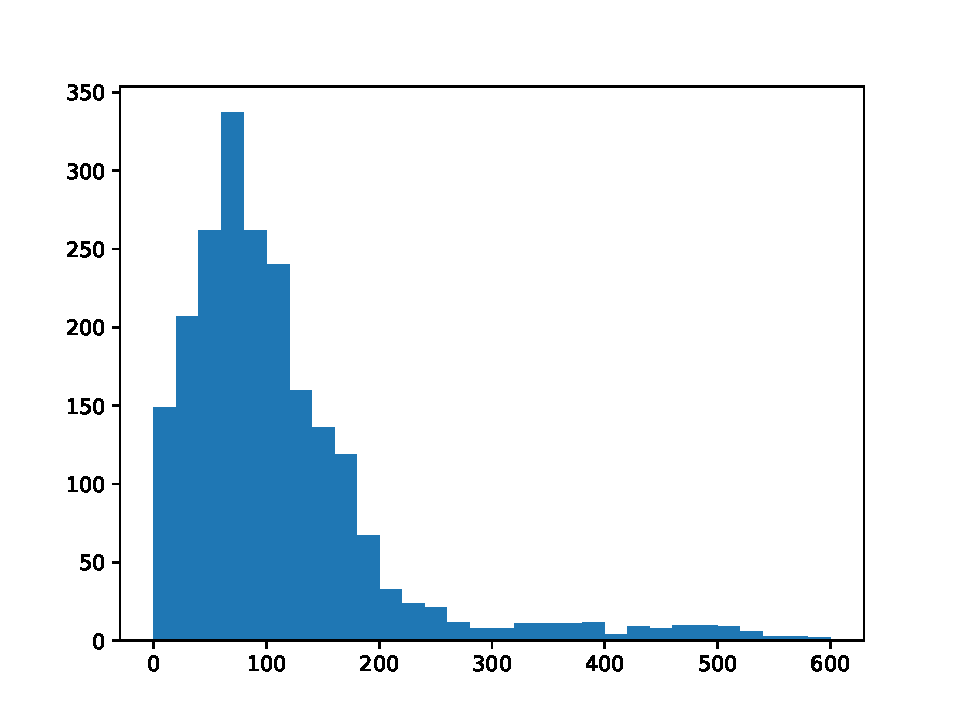
\includegraphics[width=100mm]{img/mri_cdr_offset.pdf}
    \caption{Histogram of time between MRI scans and the closest CDR assessment (in days).}
    \label{fig:mri_cdr_offset}
  \end{center}
\end{figure}

\section{Image extraction}
During the preprocessing step the three image planes are extracted from each MRI scan. For simplicity the planes chosen are simply the middle one for each axis, and the raw intensity values from each scan are flattened into the normal black/white range of PNG images.

Some scans are rotated the wrong way, even after realigning the images when loading. These images are simply skipped for now.

\section{Dataset contents}
The dataset in total contains 2782 images (ignoring the wrongly rotated ones). Of these images 20~\% were selected to be used as validation data, while the other 80~\% will be used to train the network. Just as in the paper by \textcite{islam2018early} I will use the CDR scores to divide the images into four classes: \textit{non-demented}, \textit{very mild dementia}, \textit{mild dementia}, and \textit{moderate dementia}. These classes are not equally represented in the dataset, with the more serious dementia cases being much less frequent. The total count of each case is shown in Table~\ref{tab:dataset_contents}, with the count in training and verification broken out.

\begin{table}[h]
  \begin{center}
    \caption{Count of images belonging to each class in the dataset.\label{tab:dataset_contents}}
    \begin{tabular}{r|cccc}
      \textbf{CDR Class} & \textbf{Total} & \textbf{Training set} & \textbf{Verification set} \\
      \toprule
      Non-demented (0.0) & 2163 & 1787 & 376 \\
      Very mild (0.5) & 443 & 357 & 86 \\
      Mild (1.0) & 153 & 120 & 33 \\
      Moderate (2.0) & 23 & 18 & 5 \\
    \end{tabular}
  \end{center}
\end{table}

\newpage
\section{Network structure}
\begingroup
\setlength{\columnsep}{0pt}%
\setlength\intextsep{0mm}
\begin{wrapfigure}{l}{0.3\linewidth}
  % \adjustimage{width=.3\textwidth,left}{img/model.pdf}
  \hspace*{-30mm}
	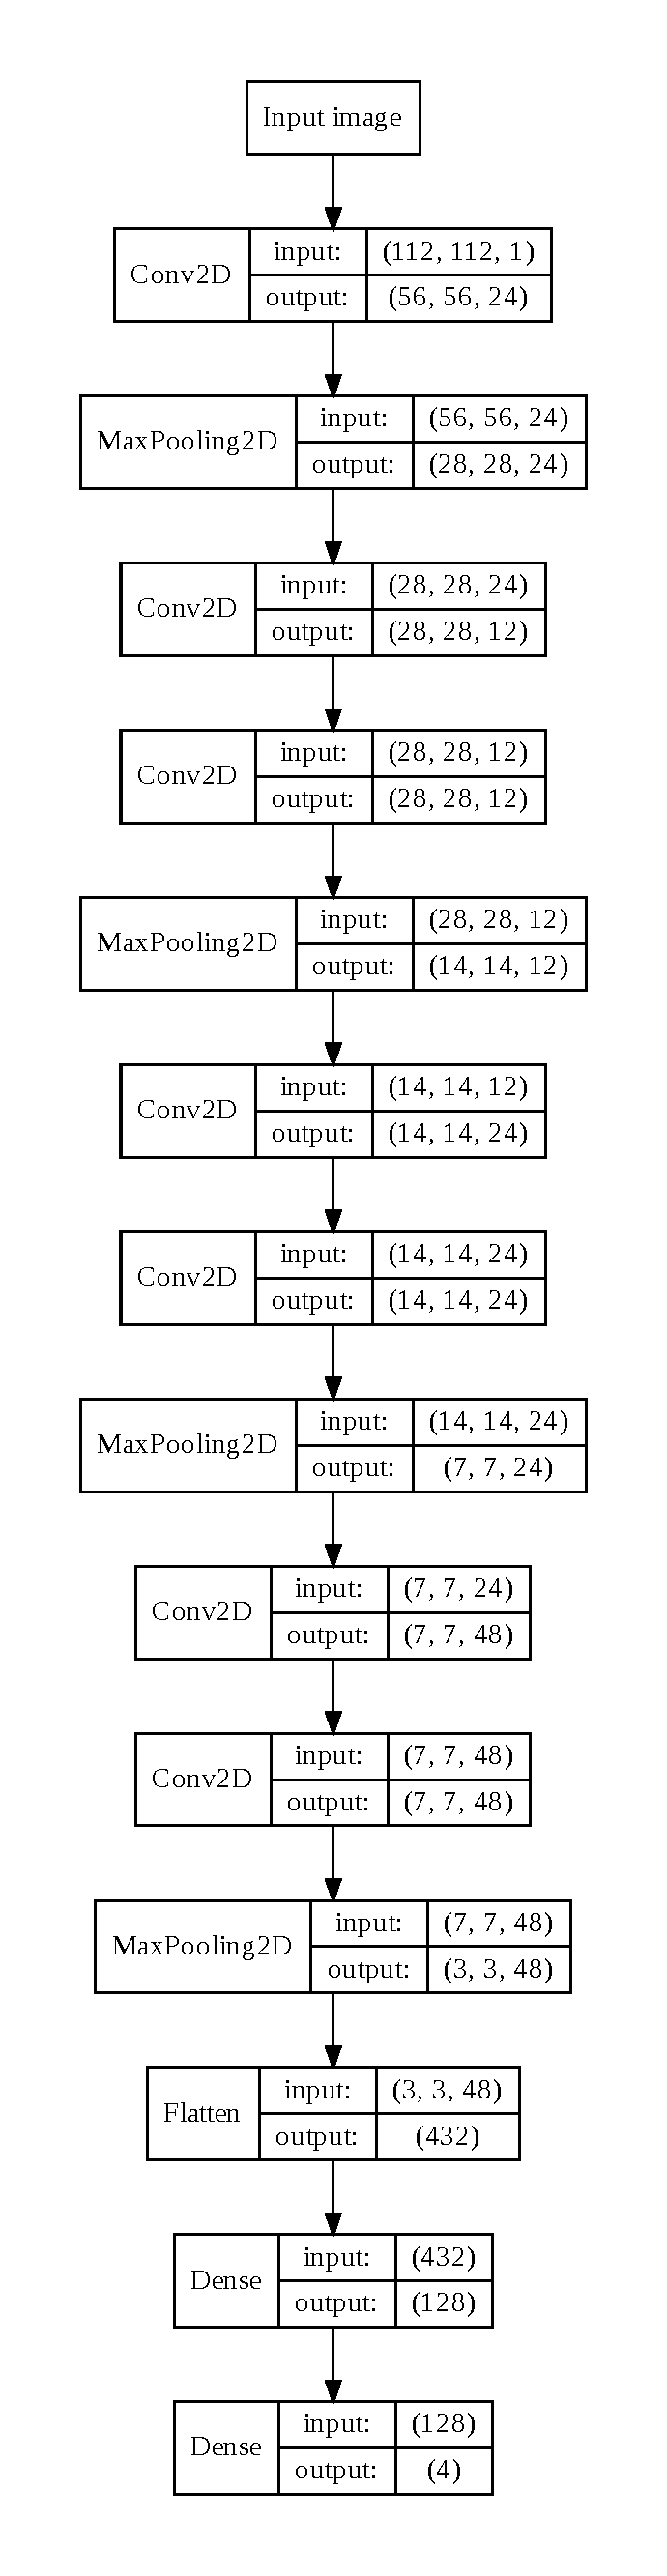
\includegraphics[width=1.7\linewidth]{img/model.pdf}
\end{wrapfigure}

We will recreate the convolutional neural network (CNN) setup used in the study by Islam and Zhang, using the machine learning framework Keras. The network will be trained and evaluated on the OASIS-3 dataset. This dataset contains data from over 2000 MRI sessions and 1000 patients, as well as medical evaluations of their disease state. OASIS-3 was a longitudinal study, which means that the imaging and evaluation of every patient was performed over a large span of time.

The dataset will be split into training, validation, and test sets, as done by Islam and Zhang. The CNN will never have seen the test set, and so it will be used for testing the accuracy. The study by Islam and Zhang resulted in a series of numerical values for accuracy, more specifically precision, recall, and f1 score. We will calculate the same values for our network trained on the larger dataset, and then compare our results with theirs. 

Studies using the smaller OASIS dataset often use cross-validation, where the training and validation is repeated multiple times so that every part of the data is used as validation at some point. This might not be possible for us depending on the computation time needed to train on the larger dataset, but would increase confidence in our results.

The CNN used by \textcite{islam2018early} uses a densely connected architecture that seems identical to DenseNet~\cite{huang2017densely}. DenseNet has implementations for both Tensorflow and PyTorch. A dense architecture means that each layer in the network is not just connected to the previous layer, but also to every other layer that came before it. This can speed up training and reduce overfitting by shrinking the parameter space and providing more direct connections between different parts of the network.

\textcite{islam2018early} do not use the entire 3D images obtained from the MRI scans. Instead, they take three slices of the image along different planes and patch them together into an image, which is then used as input to the model. It would be interesting to see if 3D convolutions could be useful for this problem, this is something we will look into if we have time.

\endgroup

\chapter{Results}
\begin{figure}
  \begin{center}
    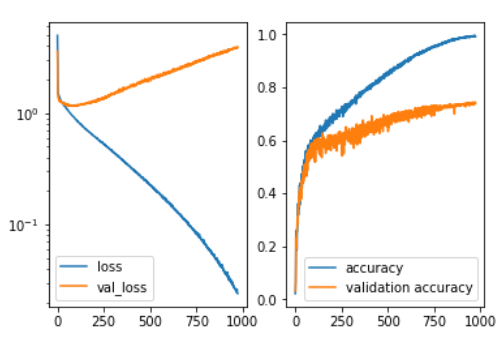
\includegraphics[width=100mm]{img/overfitted.png}
    \caption{The result when training the network for 1000 epochs without data augmentation. (Note log scale on left diagram.)}
    \label{fig:overfitted}
  \end{center}
\end{figure}
\begin{figure}
  \begin{center}
    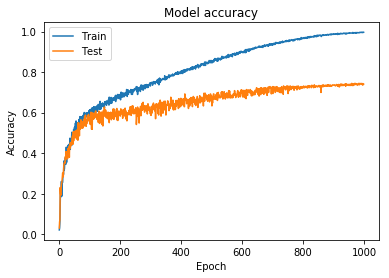
\includegraphics[width=100mm]{img/overfitted_acc.png}
    \caption{The result when training the network for 1000 epochs without data augmentation. (Note log scale on left diagram.)}
    \label{fig:overfitted_acc}
  \end{center}
\end{figure}

\begin{figure}
  \begin{subfigure}{.5\textwidth}
    \centering
    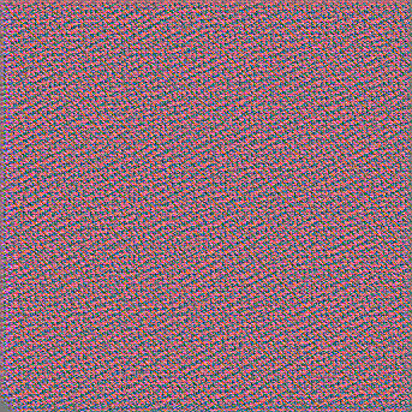
\includegraphics[width=0.9\linewidth]{img/layer0.png}
    \caption{Initial convolution}
    \label{fig:layer0}
  \end{subfigure}%
  \begin{subfigure}{.5\textwidth}
    \centering
    
\includegraphics[width=0.9\linewidth]{img/layer1.png}
    \caption{Second convolution}
    \label{fig:layer1}
  \end{subfigure}
  \\[10pt]
  \begin{subfigure}{1\textwidth}
    \centering
    
\includegraphics[width=0.45\linewidth]{img/layer2.png}
    \caption{Third convolution}
    \label{fig:layer1}
  \end{subfigure}
  \caption{Selected filter visualizations from the first three convolution layers.}
  \label{fig:filtervis}
\end{figure}

The learning rate of the Adam optimizer was found to be very important for good results. The default learning rate of $0.001$ appears to be to large, and the result was the network not improving. A lower rate of $10^{-5}$ resulted in more and faster improvement during training.

\subsection{Initial training}
At first, the network reached an accuracy of around 78~\% in a single epoch. Further training did not let the network progress.
Training the data with all classes equally, results in the op

Validating on 555 images...
              precision    recall  f1-score   support

           0       0.85      0.88      0.86       422
           1       0.39      0.32      0.35        96
           2       0.30      0.29      0.29        35
           3       0.00      0.00      0.00         2

   micro avg       0.74      0.74      0.74       555
   macro avg       0.38      0.37      0.38       555
weighted avg       0.73      0.74      0.74       555

\chapter{Discussion}
Just as in the study by \textcite{islam2018early}, the low frequency of samples in the dataset showing progressed dementia is an issue. Thanks to OASIS-3 containing many times the number of MRI images as the original OASIS does, this is not too large of a problem during training, The low frequency is however very noticible during validation, when it results in single-digit counts of the rarest class (\textit{moderate dementia}). This gives very rough knowledge of how accurate the model actually is on this type of data. It might be useful to increase the ratio of validation to training data, and in the long term create new and larger datasets that enables researchers to evaluate their models' performance with more confidence. On the other hand, detecting these progressed cases of dementia might no be very useful in practice, since by then the symptoms will be so pronounced that the diagnosis can not be missed.

\subsection{Method}
\subsection{Results}

\chapter{Conclusions}

% Print the bibliography (and make it appear in the table of contents)
\printbibliography[heading=bibintoc]

\appendix


% Tailmatter inserts the back cover page (if enabled)
\tailmatter

\end{document}
